% Esport Language (PaRa) , first experiments
% This is a rapid prototype for planning Pasigraphy Rhapsody (Paszigráfia Rapszódia, PaRa)
%
% vis_prel_para.tex
%
% Copyright (C) 2019 Norbert Bátfai, nbatfa@gmail.com, batfai.norbert@inf.unideb.hu
%
%  This program is free software: you can redistribute it and/or modify
%  it under the terms of the GNU General Public License as published by
%  the Free Software Foundation, either version 3 of the License, or
%  (at your option) any later version.
%
%  This program is distributed in the hope that it will be useful,
%  but WITHOUT ANY WARRANTY; without even the implied warranty of
%  MERCHANTABILITY or FITNESS FOR A PARTICULAR PURPOSE.  See the
%  GNU General Public License for more details.
%
%  You should have received a copy of the GNU General Public License
%  along with this program.  If not, see <https://www.gnu.org/licenses/>.
%
% Version history
%
% Initial hack
%
% vis_prel_para.tex
% Working title: Visualization of the Language of the Esports Culture: A Preliminary Study
%

\documentclass[a4paper]{article}
\usepackage[english,magyar]{babel}
\usepackage{fontspec}
\usepackage{apacite}
\usepackage{luacode}
\directlua{require('prelpara')}
\usepackage{tikz}
\usetikzlibrary{positioning}
\usepackage{url}
\usepackage{metalogo}
\usepackage{listings}
\lstset{
   breaklines=true,
   columns=flexible,
   basicstyle=\ttfamily
}
\usepackage[export]{adjustbox}
\usepackage{seqsplit}
\usepackage{csquotes}
\usepackage{graphicx}

\usetikzlibrary{shadows.blur}
\usetikzlibrary{shapes.symbols}

\definecolor{myblack}{RGB}{46,52,64}
\definecolor{mygray}{RGB}{59,66,82}
\definecolor{myorange}{RGB}{208,135,112}
\definecolor{mycyan}{RGB}{94,129,172}
\definecolor{myyellow}{RGB}{235,203,139}
\definecolor{mypink}{RGB}{180,142,173}

\newcommand{\paradump}[1]{{\ttfamily\seqsplit{#1}}}

\newcommand\N[1]{\directlua{N(#1) }}
\newcommand\D[3]{\directlua{D(#1,#2,#3) }}
\newcommand\prelparaIID[1]{\directlua{para2D(#1)}}
\newcommand\prelparaIIID[2]{\directlua{para3D(#1,#2)}}

\begin{document}

\title{Az esport kultúra nyelvének vizualizációja: egy el\H otanulmány\\Visualization of the Language of the Esports Culture: A Preliminary Study}
\author{
	Bátfai Norbert\\
	\texttt{batfai.norbert@inf.unideb.hu}}
\date{
    Információ Technológia Tanszék, Debreceni Egyetem, Magyarország\\
    \today
}

\maketitle

\begin{abstract}
A Paszigráfia Rapszódia \cite{PARAREPO}, vagy röviden PaRa egy olyan mesterséges nyelv kialakítására törekv\H o kezdeményezés, mely lehetővé teszi a homunkulusz és a mesterséges homunkulusz közötti kommunikációt, ergó ez az esport kultúra nyelve \cite{MITEL}. Ebben az el\H otanulmányban a PaRa vizualizációs lehetőségeit vizsgáljuk. Ennek alapjai az SMNIST \cite{SMNIST} képekb\H ol származnak, ahol a képeken lév\H o pöttyök számosságát kell meghatározni. Ám meg kell jegyezzük, hogy a PaRa esetében nem a számosság, hanem a pöttyök pontos helyzete a meghatározó.
\end{abstract}

{
\selectlanguage{english}
\begin{abstract}
The Pasigraphy Rhapsody \cite{PARAREPO}, or shortly PaRa (from it's Hungarian name Paszigr\'afia Rapsz\'odia) is an initiative to develop an artificial language that is intended to allow communication between the Homunculus and the Artificial Homunculus, ergo, it is the language of the esport culture \cite{MITEL}. In this preliminary study, we investigate some possibilities of visualization of Pasigraphy Rhapsody. Its intuitive base comes from SMNIST images \cite{SMNIST}, where the numerosity of dots must be recognized in images. But it should be noticed that in this case the numerosity does not matter but the exact position of the dots.
\end{abstract}
}

\section{Introduction}

The sentences of PaRa are n-dimensional hypercubes \cite{CONPARA}.

\subsection{First Attemptions}

\subsubsection{A 2D \LuaLaTeX -based visualization}


\noindent
\begin{tikzpicture}[thick,scale=2, every node/.style={scale=2}]
\prelparaIID{"4:8:3:0:1:2:2:3:4:10:2:0:9:9:1:8:4:2:2:5:2:1:6:4:4:6:2:1:5:5:1"}
\end{tikzpicture}

\paradump{4:8:3:0:1:2:2:3:4:10:2:0:9:9:1:8:4:2:2:5:2:1:6:4:4:6:2:1:5:5:1}

\noindent
\begin{tikzpicture}[thick,scale=2, every node/.style={scale=2}]
\prelparaIID{"3:4:1:1:1:8:2:2:2:4:4:2:1:1:1"}
\end{tikzpicture}

\paradump{3:4:1:1:1:8:2:2:2:4:4:2:1:1:1}

\subsubsection{A 3D \LuaLaTeX -based visualization}

At the moment, we are experimenting with multiple TikZ based visualizations. The first one uses slant\footnote{The idea of using yslant and xslant to achieve a 3D effect like appearance comes from Stefan Kottwitz's \textquote{Sudoku 3D cube} example \url{http://www.texample.net/tikz/examples/sudoku-3d-cube/}.} and shift transformations.

\begin{tikzpicture}[thick, scale=2, every node/.style={scale=2}]
\prelparaIIID{1}{"3:4:3:0:1:2:2:3:4:10:2:0:9:9:0:8:2:1:6:6:1:6:2:1:5:5:1:8:2:1:7:7:1:4:2:1:3:3:1:4:2:1:3:3:1:10:2:1:7:7:1:6:2:1:5:5:1"}
\prelparaIIID{2} {"4:4:3:1:2:2:2:3:4:10:2:0:9:9:0:8:2:1:6:6:1:6:2:1:5:5:1:8:2:1:7:7:1:4:2:1:3:3:1:4:2:1:3:3:1:2:1:1:1:6:2:1:5:5:1:4:1:1:1:8:2:2:2:4:4:2:1:1:1"}
\prelparaIIID{1}{"3:4:3:0:1:2:2:3:4:10:2:0:9:9:0:8:2:1:6:6:1:6:2:1:5:5:1:8:2:1:7:7:1:4:2:1:3:3:1:4:2:1:3:3:1:10:2:1:7:7:1:6:2:1:5:5:1"}
\end{tikzpicture}


\begin{tikzpicture}
\prelparaIIID{1}{"3:4:3:0:1:2:2:3:4:10:2:0:9:9:0:8:2:1:6:6:1:6:2:1:5:5:1:8:2:1:7:7:1:4:2:1:3:3:1:4:2:1:3:3:1:10:2:1:7:7:1:6:2:1:5:5:1"}
\prelparaIIID{2} {"4:4:3:1:2:2:2:3:4:10:2:0:9:9:0:8:2:1:6:6:1:6:2:1:5:5:1:8:2:1:7:7:1:4:2:1:3:3:1:4:2:1:3:3:1:2:1:1:1:6:2:1:5:5:1:4:1:1:1:8:2:2:2:4:4:2:1:1:1"}
\end{tikzpicture}

\begin{tikzpicture}
\prelparaIIID{1} {"4:4:3:1:2:2:2:3:4:10:2:0:9:9:0:8:2:1:6:6:1:6:2:1:5:5:1:8:2:1:7:7:1:4:2:1:3:3:1:4:2:1:3:3:1:2:1:1:1:6:2:1:5:5:1:4:1:1:1:8:2:2:2:4:4:2:1:1:1"}
\prelparaIIID{2}{"3:4:3:0:1:2:2:3:4:10:2:0:9:9:0:8:2:1:6:6:1:6:2:1:5:5:1:8:2:1:7:7:1:4:2:1:3:3:1:4:2:1:3:3:1:10:2:1:7:7:1:6:2:1:5:5:1"}
\end{tikzpicture}

\begin{tikzpicture}
\prelparaIIID{1}{"4:8:3:0:1:2:2:3:4:10:2:0:9:9:0:8:2:1:6:6:1:6:2:1:5:5:1:8:2:1:7:7:1:4:2:1:3:3:1:4:2:1:3:3:1:10:2:1:7:7:1:6:2:1:5:5:1:4:1:1:1:8:2:2:2:4:4:2:1:1:1"}
\end{tikzpicture}

\subsubsection{An OpenGL based visualization}

\paradump{./para6 \  3:2:1:1:0:3:2:1:0:2:0:2:1:1:0:3:3:0:2:0:1:1:0:1:0:1:0:1:0:2:2:0:1:1:1:3:2:1:0:2:0:2:1:1:1:2:3:0:1:1:1:1:0:3:3:0:1:0:2:1:0:1:0:2:2:0:0:0:1:3:1:0:1:3:2:1:0:2:0:3:3:0:1:0:2:1:0}

\begin{figure}[h]
\begin{tabular}{ll}
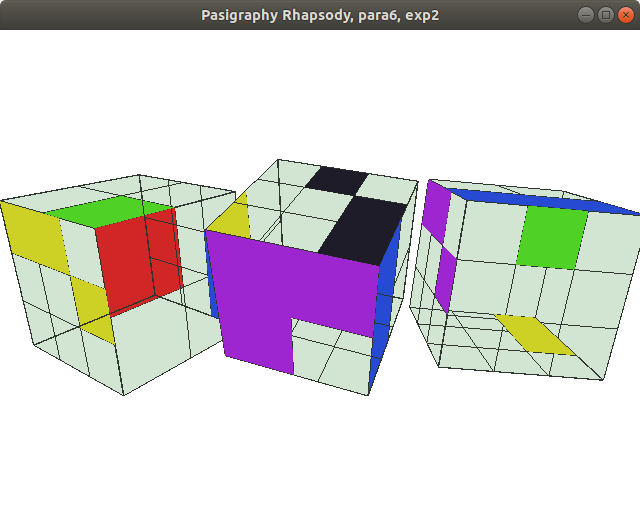
\includegraphics[scale=.25, frame]{para6exp2t}
&
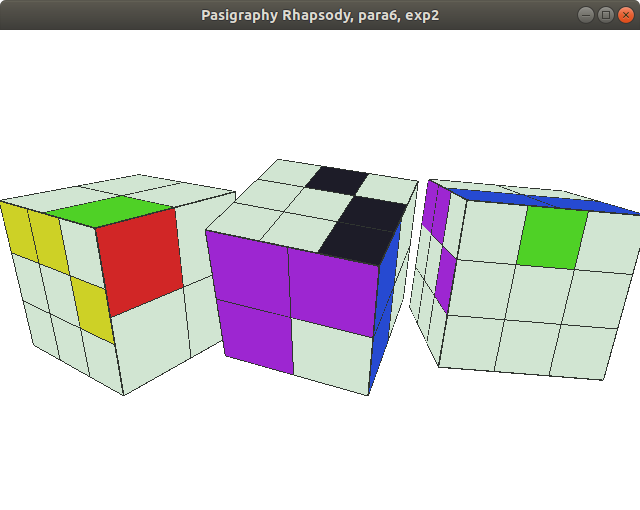
\includegraphics[scale=.25, frame]{para6exp2}
\end{tabular}
\caption{Cube letters can be rotated separately around all three directions. A négyzet betűk mindhárom irányban külön forgathatóak. Az adott betű kijelölése nehézkes.}
\label{figpara6}
\end{figure}


\begin{figure}[h]
\begin{tabular}{ll}
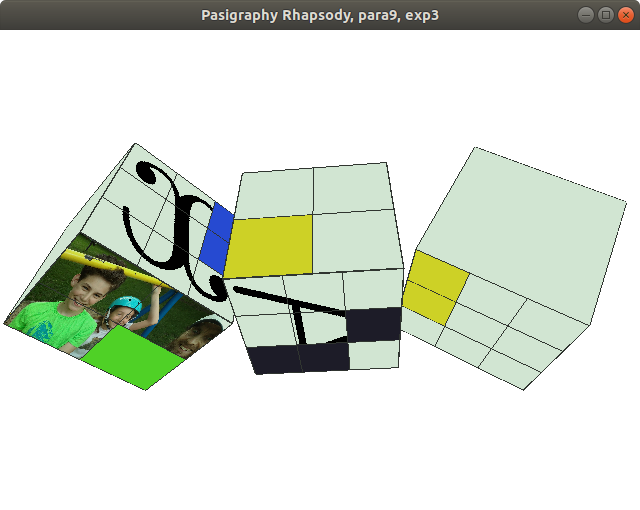
\includegraphics[scale=.25, frame]{para9}
&
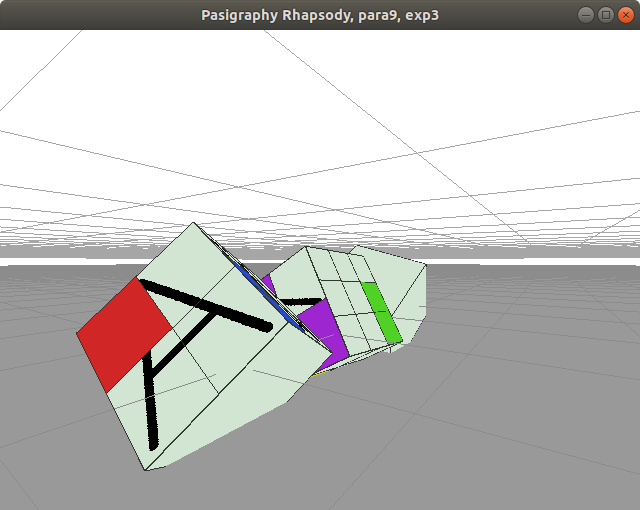
\includegraphics[scale=.25, frame]{para92}
\end{tabular}
\caption{We may use texture pictures for cube letters that are organized in stacked floors and the floors together can be rotated around all three directions. Textúrázhatjuk a négyzet betűket, melyek egymásra épülő emeletekbe vannak szervezve, ahol az emeletek együtt mindhárom irányban forgathatóak.}
\label{figpara9}
\end{figure}

\begin{figure}[h]
\begin{tabular}{ll}
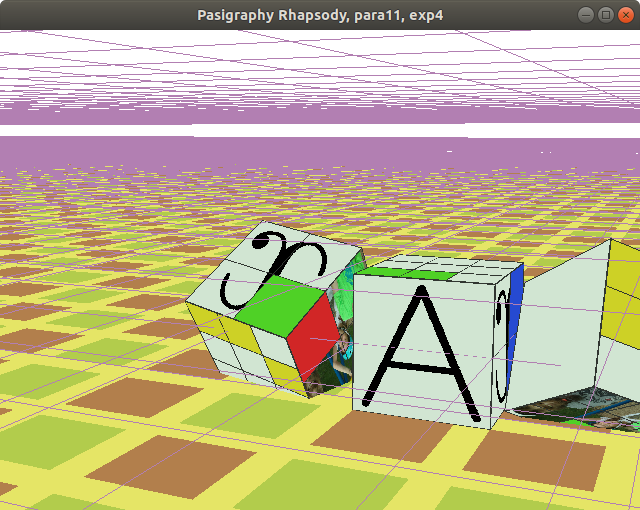
\includegraphics[scale=.25, frame]{para112}
&
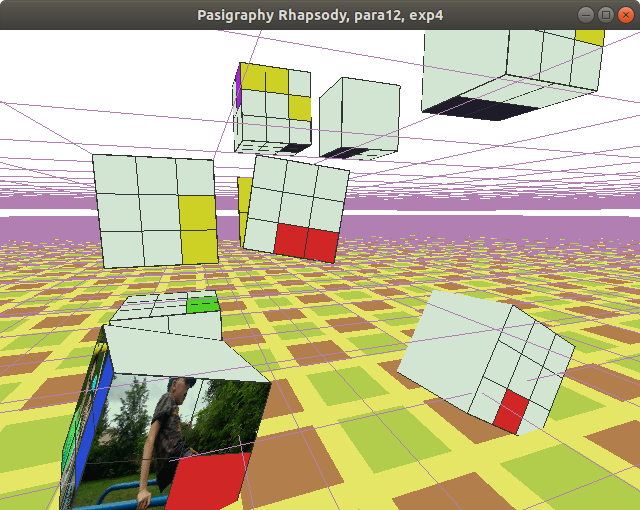
\includegraphics[scale=.25, frame]{para11}
\end{tabular}
\caption{On a given floor we can move with WASD as is usual in FPS. Adott emeleten az FPS-ekben szokásos WASD gombokkal mozgunk. Az FPS jellegből adódik a betűk könnyedebb kijelölése: az van kiválasztva, amelyik a legközelebb van hozzánk, vagy amelyikre nézünk.}
\label{figpara6}
\end{figure}

\bibliographystyle{apacite}
\bibliography{prel_para}

\section*{License}

{\footnotesize
\begin{verbatim}
% Copyright (C) 2019 Norbert Bátfai
% nbatfa@gmail.com, batfai.norbert@inf.unideb.hu
%
%  This program is free software: you can redistribute it and/or modify
%  it under the terms of the GNU General Public License as published by
%  the Free Software Foundation, either version 3 of the License, or
%  (at your option) any later version.
%
%  This program is distributed in the hope that it will be useful,
%  but WITHOUT ANY WARRANTY; without even the implied warranty of
%  MERCHANTABILITY or FITNESS FOR A PARTICULAR PURPOSE.  See the
%  GNU General Public License for more details.
%
%  You should have received a copy of the GNU General Public License
%  along with this program.  If not, see <https://www.gnu.org/licenses/>.
\end{verbatim}
}

\end{document}
